\chapter{TROPOS Methodology with Probabilistic Requirements Verification}\label{ch:proposal}

This chapter describes the extended TROPOS methodology applied to the MPERS case study. Both TROPOS early and late requirements analysis phases are fully presented, as well as the verification process that requires a behaviour specification and the additional contextual notation regarding context effects. Further details about the TROPOS methodology may be found in the reference literature~[TROPOS]. 

\section{TROPOS Requirements Engineering Phases}

\subsection{TROPOS Early Requirements Phase}

In Early Requirements phase, stakeholders are modelled as as well as their needs. Each actor may be a depender or a dependee of a goal, task or resource dependency. In this phase, only the main system actor and the application domain stakeholders are analysed, leaving the detailed system analysis to later development phases.

The MPERS sytem and its social dependencies are presented by the actor model in Figure~\ref{fig:MPERS_ER}. System actors and social actors are displayed in different colors. Among the stakeholders, the emergency center represents a private or public organization interested in providing an emergency response service to patients. Patient and doctor represent, respectively, the assisted person and the medical responsible for defining and evolving the emergency detection rules as part of an evolutionary approach for personal emergency response. Finally, sensors retailer should provide the vital signs sensors required for monitoring.

\begin{figure*}[ht]
\centering
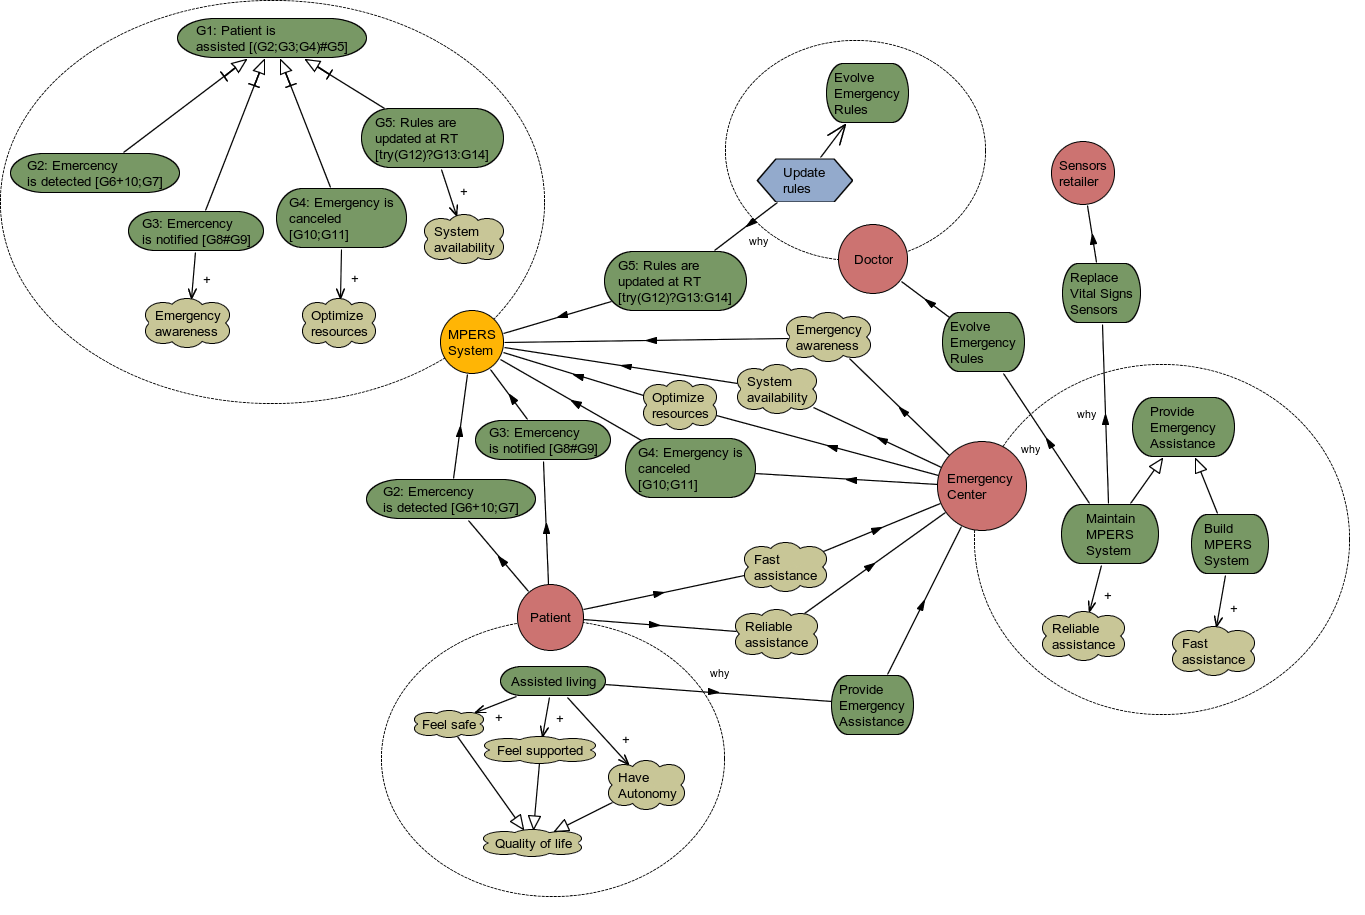
\includegraphics[width=1\textwidth]{imgs/MPERS_ER.png}
\caption{MPERS at TROPOS early requirements phase}
\label{fig:MPERS_ER}
\end{figure*}

From the diagram in Figure~\ref{fig:MPERS_ER} it is possible to have a first view of the MPERS system-to-be. Main goals are divided in detecting, notifying and checking an emergency. Also, the ability to update the emergency rules at runtime (RT) is the fourth and last mandatory goal (AND-decomposition) that fulfils the `Patient is assisted' root goal. System goals are directly or indirectly related to stakeholders functional and non-functional needs.

The yellow circle indicates that MPERS is a system actor. MPERS goals can be seen with a regex indicating its dynamic behaviour as part of the runtime goal model specification required by the proposal. This notation is a reflex of the late requirements phase, as the TAOM4E tool supporting TROPOS methodology shares unique entities and relations among different development phases. The regex syntax is enclosed by brackets to differentiate then from goal name. In future work, a specific modelling compartment should receive the values for the runtime regex.

\subsection{TROPOS Late Requirements Phase}

Later requirements phase concentrates the analysis in the system-to-be and its operational environment. The MPERS goal model occupies the most part of the diagram and each of its main goals are further decomposed through AND/OR decomposition. Also, means-end tasks defines how leaf-goals are fulfilled and the runtime regex across goals and tasks specifies dynamic properties of the system-to-be behaviour. Figure~\ref{fig:MPERS_LR} illustrates the late requirements diagram for the MPERS.

\begin{figure*}[h!]
\centering
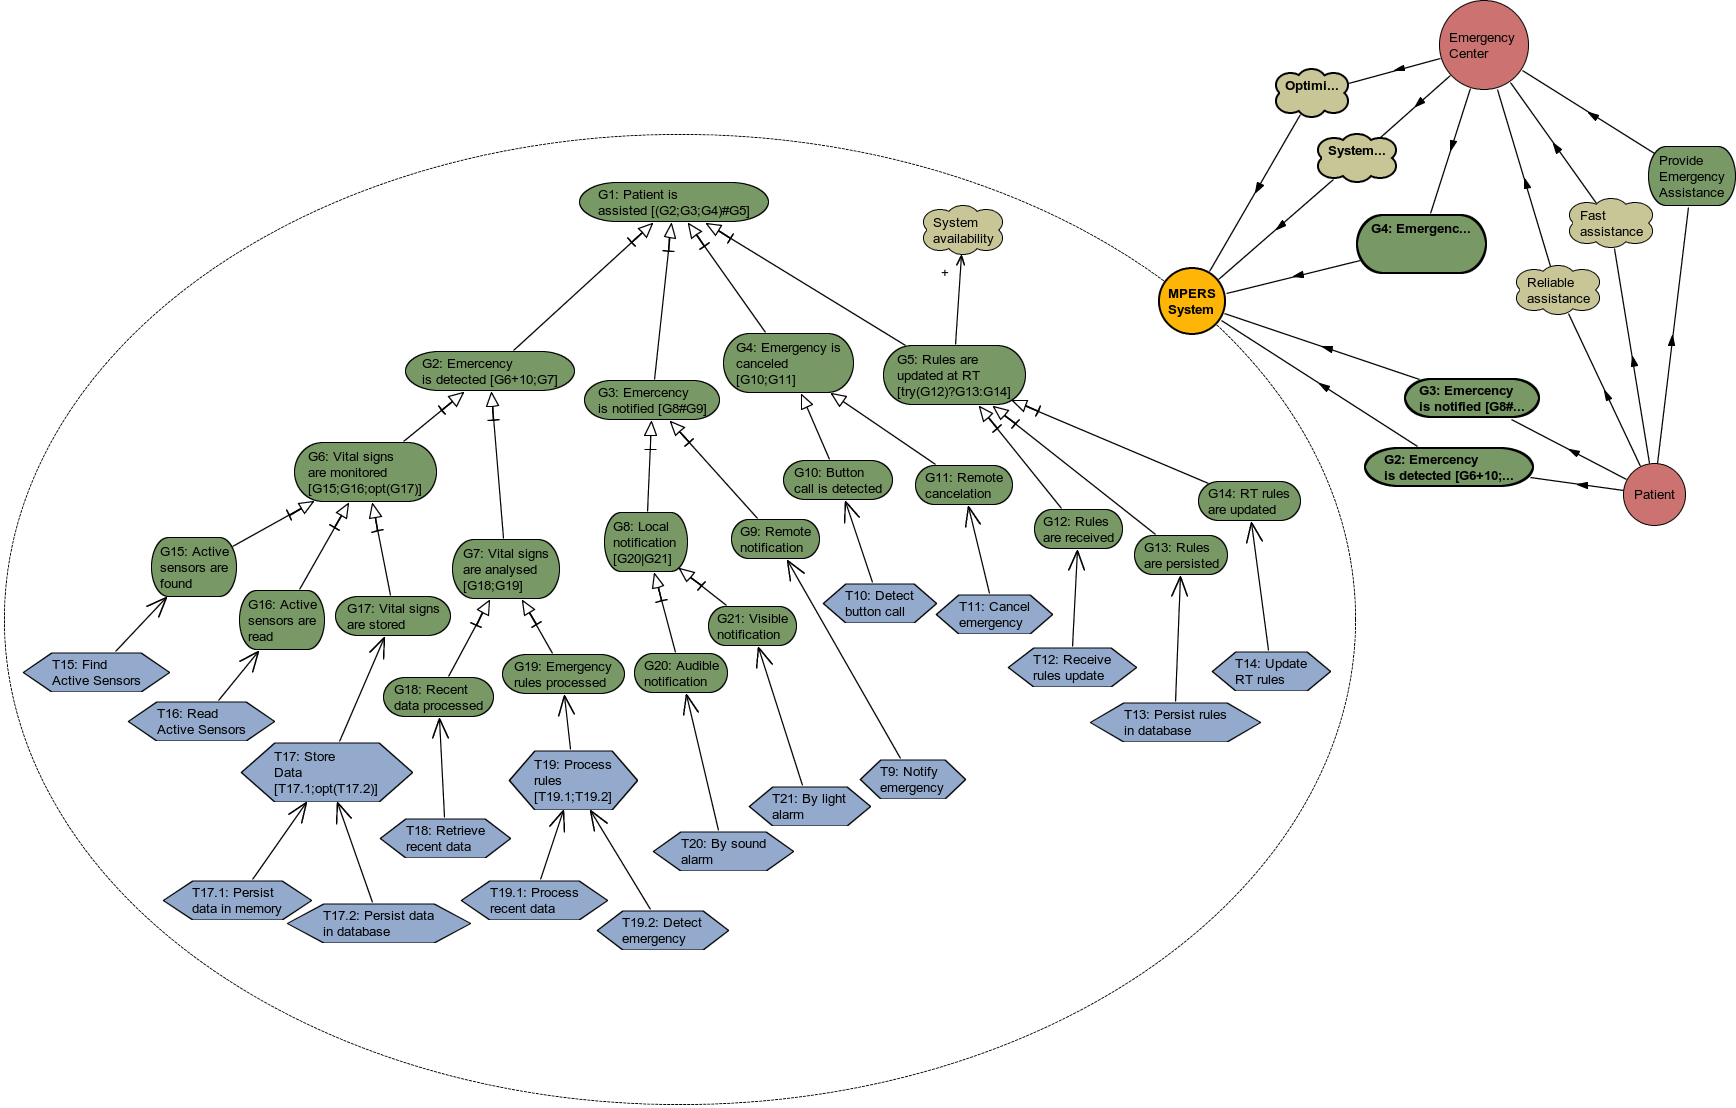
\includegraphics[width=1\textwidth]{imgs/MPERS_LR.png}
\caption{MPERS at TROPOS early requirements phase}
\label{fig:MPERS_LR}
\end{figure*}

At this stage of the methodology, the system is represented as a monolithic actor and its goal model may be extended with the runtime specification. This extended model merges multiple views in the same diagram: goals and tasks represent the requirements view for the system-to-be as well as the intentionality behind then, while the runtime specification provides a dynamic representation in terms of goal achievement  and task execution.

In this work, we have first explored the use of the PMC technique for the verification of dependability attributes in the system model of the TROPOS late requirements phase. The idea is to initially evaluate the approach in a monolithic representation without the additional complexity of a multi-agent architecture. The evaluation involving later TROPOS phases should be explored in future work. The remaining of this section will focus on the extended verification phase proposed by this work.

\section{TROPOS Extended Verification Phase}

%To evaluate our verification approach with the MPERS case study, we have used a discrete-time Markov chain (DTMC) probabilistic model and focused on the verification of NFR related to dependability, i.e., NFR that are either direct attributes encompassed by dependability or that are related to one or more of these attributes.

In this section, the TROPOS extension for NFR verification using a PMC technique is presented. First, non-functional constraints are associated to the MPERS goal model. Then, the runtime regex is further detailed and compared to a UML activity diagram. After this, the high-level DTMC model is built and details about the conversion from a RGM to a DTMC are provided. Finally, we demonstrate how to estimate reliability of the RGM based on individual reliability of leaf-tasks mapped to the DTMC model.

Figure~\ref{fig:CRGM_TO_DTMC} illustrates the extended TROPOS methodology that starts with original phases involving goal-oriented modelling and ends with the generation of a high-level DTMC model used for the verification of NFRs as the MPERS global reliability.

\begin{figure*}[h!]
\centering
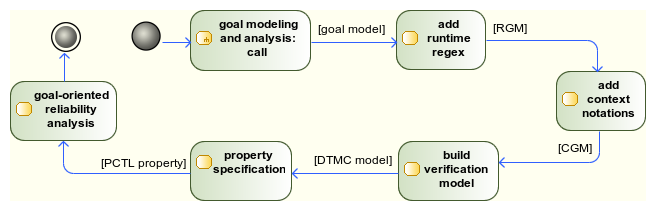
\includegraphics[width=0.60\textwidth]{imgs/CRGM_TO_DTMC.png}
\caption{Building a DTMC model from a contextual/runtime goal model.}
\label{fig:CRGM_TO_DTMC}
\end{figure*}

\subsection{Non-functional requirements specification}

TROPOS goal model also provides rationale for NFR analysis, as it originally inherited the softgoal analysis from the NFR framework~[NFR]. In our approach, non-functional constraints are modelled as qualitative hard goals with a clear cut value for its satisfaction, complementing the other NFRs modelled as softgoals. As a benefit of a goal-oriented modelling for NFRs, the elicitation of a given NFR may be justified by its relation to other elements in the model. Figure~\ref{fig:MPERS_NFR} presents some NFRs for the MPERS system actor.

\begin{figure*}[h!]
\centering
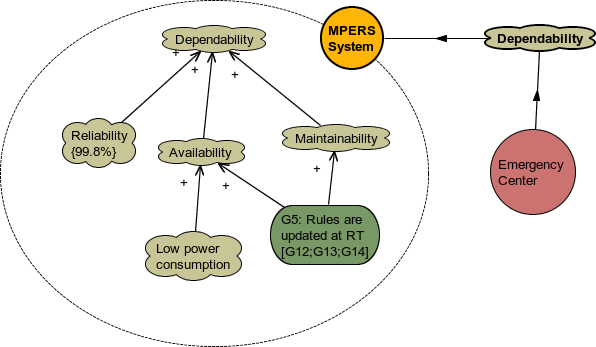
\includegraphics[width=0.6\textwidth]{imgs/MPERS_NFR.png}
\caption{MPERS non-functional requirements.}
\label{fig:MPERS_NFR}
\end{figure*}

%Intersting for motivation!
Similarly to the Awareness Requirements by Souza et al.~[AWREQ], some NFR define metrics over other requirements. These meta-requirements are not directly fulfilled by system functionalities like `emergency awareness' is fulfilled by `notify emergency' or `confidentiality' could be fulfilled by `user authentication', but by how these functionalities will perform. Reliability, for instance, is inversely proportional to the likelihood of failures. Hence, the reliability metric depends on the probability of system functionalities to fail. Conformity to these metrics is not implicit in the model, it requires some verification technique.

%PUT a goal model with hard goal NFRs!

%PUT SOME NFR CONCEPTUAL MODEL HERE!

Each requirement in a goal model must come from another requirement through decomposition, means-end or contribution links, or it must be directly mapped to stakeholder needs through dependency links. Emergency center attended the patient's needs by providing and maintaining the MPERS system itself and by assuring other NFR for the system. Availability and reliability were selected as metrics over the system execution (meta-requirement), while maintainability is partially satisfied by the MPERS ability to update emergency rules at runtime and by other aspects that, for the sake of simplicity, we will omit in this evaluation.

The specification of non-functional constraints is a sensible task that depends on expertise and on domain knowledge. For instance, an analyst or a reliability engineer should be aware of what does it mean for a system to be 99.999\% reliable, as this level may not be achieved by any alternative solution and must be coherent to the system criticality - a catastrophic failure should be avoided by all means. In some cases, the system will have to comply to some industry standards or contract based constraints. Table~\ref{tab:MPERS_NFR} summarizes two possible non-functional constraints for the MPERS.
\medskip

% Please add the following required packages to your document preamble:
% \usepackage{booktabs}
\begin{table}[h]
{\renewcommand{\arraystretch}{1.5}
\begin{tabularx}{\textwidth}{@{}XXX@{}}
\toprule
\textbf{NFR}               & \textbf{Constraint} & \textbf{Target}        \\ \midrule
\textbf{Reliability}       & 99.8\%            & \textbf{G1} \\
\textbf{Power consumption} & 100 p.u.            & \textbf{G2}          \\ \bottomrule
\end{tabularx}
}
\caption{Non-functional metrics for the MPERS system.}
\label{tab:MPERS_NFR}
\end{table}

%softgoals of `continuous assistance' and `correct assistance'

As indicated by the \textit{Target} column, each NFR constraint may be associated to a root level goal or to any of its subgoals. The corresponding probabilistic verification based on the execution of a set of leaf-tasks in the RGM is defined as:

\begin{itemize}

\item \textit{Global}, if the activities set is a minimum set composed of the tasks that satisfies the chain of subgoals up to the root goal Groot. For instance, in Table~\ref{tab:MPERS_NFR} reliability is associated to root goal G1.
\medskip

\item \textit{Local}, if the activities set is a minimum set composed of tasks that satisfies the chain of subgoals up to a goal Gx, where Gx != Groot. For instance, in Table~\ref{tab:MPERS_NFR}, power consumption is (locally) associated to goal G2.
\medskip

\end{itemize}

%put here the formal definition of the root goal, subgoals, activity set, turple, etc

Other MPERS NFR are `emergency awareness' and `resources optimization'. These softgoals are addressed by system functionalities. The former receives a full contribution (double positive sign) from goal `emergency is notified', meaning it is fully satisfied by this goal. The later is just assumed to be partially satisfied by the `emergency is checked' functional goal.

\subsection{Behaviour specification}

In this section, further details about the runtime regex syntax and semantic will be explained as they are a central part of this proposal. Table~\ref{tab:RGM_REGEX} provides a textual description of each RGM notation with corresponding meaning in terms of what behaviour it specifies and also an example from the MPERS RGM. A formal and detailed description can be found in the RGM reference publication~[RGM].

% Please add the following required packages to your document preamble:
% \usepackage{booktabs}
\begin{table}[h]
{\renewcommand{\arraystretch}{1.5}
\begin{tabularx}{\textwidth}{@{}l|X|X@{}}
\toprule
\textbf{Expression} & \textbf{Meaning}                                                                   & \textbf{Example (MPERS)} \\ 
skip                & No action. Useful for conditional ternary expressions involving two elements.      & try(G10)?skip:G11        \\ 
E1;E2               & A goal/task E1 must be fulfilled/executed before E2.                               & G1;G2;G3                 \\ 
E1|E2               & Fulfillment/execution of goal/task E1 is alternative with respect to E2. & T9.1|T9.2                \\ 
opt(E)              & Fulfillment/execution of goal/task E is not mandatory.                             & opt(T17.2)               \\ 
E+n                 & Goal/task E must be fulfilled/executed n times, with n \textgreater 0.             & G22+2                    \\ 
try(E)?E1:E2        & If goal/task E succeeds, E1 must be fulfilled/executed; otherwise, E2.             & try(G10)?skip:G11        \\ 
E1\#E2              & Interleaved fulfillment/execution of goal/task E1 and E2.                          & G8\#G9                   \\ 
E\#n                & Interleaved fulfillment/execution of n instances of E, with n \textgreater 0.      & -                        \\ \bottomrule
\end{tabularx}
}
\caption{Description of RGM textual notations used by the proposal.}
\label{tab:RGM_REGEX}
\end{table}

A small variation of the original regex was employed for the E+ and E\# rules. Instead of an undetermined number of goal/task instances, analyst should provide the exact number of instances for goals achievement and tasks execution. This information is required for the generation of the verification model from a RGM.

\subsubsection{RGM - UML activity diagram comparison}\label{ssec:RGM-UML}

A similar specification could be provided by an UML activity diagram with activities as leaf-tasks of the goal model. However, activity diagrams have an homogeneous abstraction level and do not clearly correlate behaviour to the requirements they are meant to satisfy. In contrast to the RGM, activity diagrams denote behaviour through graphical symbols, while the RGM mixes the original goal model notation with a runtime regex. This simple notation increases the utility of a goal model diagram. Figure~\ref{fig:MPERS_UMLAD} presents an activity diagram corresponding to the MPERS RGM. 

\begin{figure*}[h!]
\centering
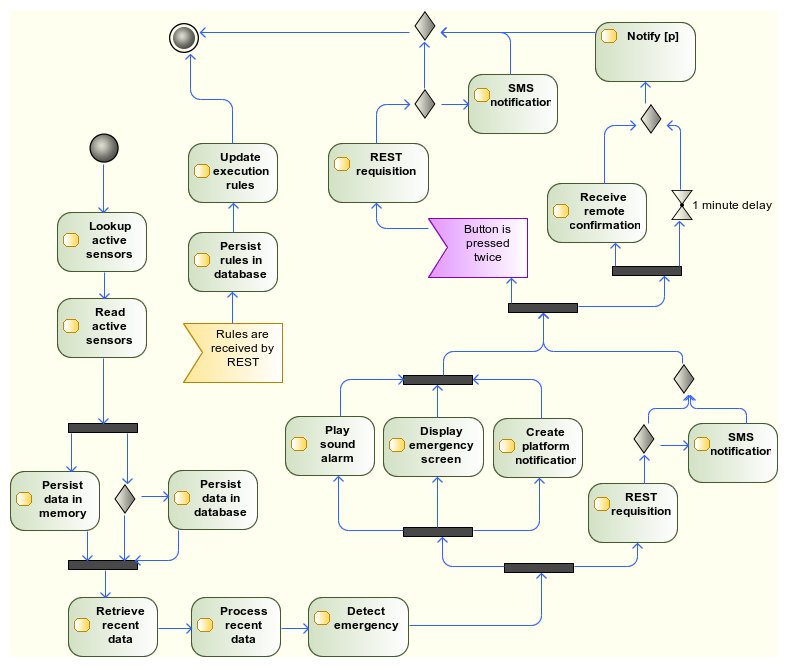
\includegraphics[width=1\textwidth]{imgs/MPERS_UMLAD.png}
\caption{MPERS tasks represented by a UML activity diagram}
\label{fig:MPERS_UMLAD}
\end{figure*}

Among its limitations, RGM does not express that an emergency has to be confirmed after a time or signal event as the UML activity diagram does. Both necessary and sufficient conditions for the triggering and fulfilment of goals, tasks and dependencies are provided by Formal TROPOS language.  Still, sequential, parallel, alternative, optional and conditional execution flows as long as multiple executions of the same task can be expressed by the RGM, providing a rich behaviour specification that could be checked for non-functional requirements such as dependability attributes.

The idea of a runtime goal model is not to replace UML activity diagrams, but to complement the static goal model with a clear runtime syntax that could be used for 
communication and for conformance verification at both design time and during system execution - as the execution monitoring originally proposed by Dalpiaz et al~[RGM]. Depending on the complexity of the behaviour specification, a more robust runtime syntax would have to be employed or a standard UML behaviour diagram such as activity and sequence diagrams would have to complement the goal model.

\subsection{Non-functional requirements verification}

%NOT HERE!
%The probabilistic verification of systems with variability is not a novelty by itself. Many proposals have addressed this problem in the context of Dynamic Software Product Lines (DSPL), some of then using the PMC technique~[Vini, Paula, Who Else?]. In DSPL, optional and alternative features may be activated or deactivated at runtime. A family based verification of one or multiple NFRs, also called qualitative goals, indicates what combinations are valid or which combination is optimal.

This section describes the application of a PMC technique to verify the conformance of the RGM to defined non-functional constraints and also to solve the variability problem at design time considering both cases explained in Section~\ref{sec:variability}, i.e., for static context and dynamic contexts.

\subsubsection{Leaf-tasks as DTMC modules}

%It is not always the case that multiple alternatives must be evaluated and compared. A goal model may be built with only mandatory goals, dependencies and tasks. Nonetheless, non-functional constraints may still have to be checked, i.e., a single alternative verification may have to be performed. 

The state-based verification of meta-requirements or non-functional constraints that specifies how different functionalities should perform is a complex task that involves a representation of system states and their transitions. A goal model may define system requirements with variable abstraction levels. As such, the feasibility of the verification of a given metric depends on the information provided by the model.

The MPERS RGM in Figure~\ref{fig:MPERS_LR} expands its main goals in further subgoals that are ultimately satisfied by operational tasks. Tasks can also be expanded in more granular subtasks. Tasks without outgoing relations are named leaf-tasks. In our proposal, leaf-tasks are mapped to modules in a DTMC model in PRISM language. PRISM modules are containers for variables and commands, i.e., for states and behaviour. Figure~\ref{fig:PRISM_TASK_MODULE} presents a system task as a PRISM module.

%TODO: REMOVE THE RELIABILITY VALUE
\begin{figure*}[ht]
\centering
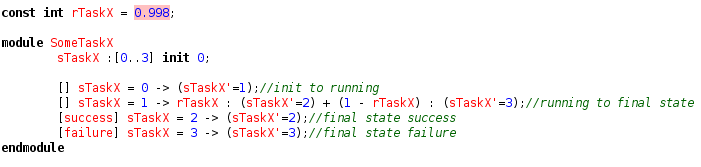
\includegraphics[width=1\textwidth]{imgs/PRISM_TASK_MODULE.png}
\caption{A PRISM DTMC module representing a system task.}
\label{fig:PRISM_TASK_MODULE}
\end{figure*}

In the DTMC model, leaf-tasks have their execution state mapped to a variable in the model (sTask variable in Figure~\ref{fig:PRISM_TASK_MODULE}). From the RGM original set of goal/tasks instance states, we considered the following values:

\begin{itemize}

\item Init(sTask=0): corresponds to the initial state of a given leaf-task. From this state, a transition may occur to the running state, if this task is part of a system alternative that will be analysed, or directly to the final success state, if the opposite.
\medskip

\item Running(sTask=1): corresponds to the operational state of a given leaf-task. From this state, a transition to the final success or failure states may occur. A variable rTask ranging from 0 - 1 defines the task's reliability, i.e., the probability of a transition to the success state - and the complementary transition probability to the failure state.
\medskip

\item Success(sTask=2): corresponds to the absorbing final state of success of a singular task execution.
\medskip

\item Failure(sTask=3): the opposite from the final success state.

\end{itemize}

%init (0), running (1), success (2) and failure (3). Success and failure are the final absorbing states for a task instance. Transition to these states is conditioned to the rTask probability: the closer this variable is to 1, the higher the probability of reaching the success state. 


\subsubsection{Building the high-level DTMC model from a RGM}


Given a set of leaf-tasks that fulfils a chain of subgoals until a certain goal G, a DTMC model composed of modules for each leaf-task states and transitions is build. This model must represent the same workflow of the corresponding RGM.  

In this work, we are not interested in checking system instance conformance to its runtime goal model through monitoring as the original RGM proposal. We focus on the estimation of non-functional metrics based on the high-level DTMC model. We call it a high-level DTMC model because leaf-tasks are similar to activities in a UML diagram whose behaviour could be further detailed, e.g., by sequence diagrams.

Each leaf-task in the DTMC model starts at a discrete time slot. Time slots defines the sequence order of tasks executions. Sequential tasks (T1;T2) have subsequent time slots, meaning that T2's initial transition is synchronized to T1's final transition. Interleaved tasks (T1\#T2) have their initial state transition synchronized at the same time slot through labels, but occupy different time paths, i.e., following state transitions are interleaved.  Figure~\ref{fig:UML_SEQ_TSKS} and~\ref{fig:UML_PAR_TSKS} present sequence and interleaved execution cases in UML notation.

\begin{figure}
        \centering
        \begin{subfigure}[b]{0.4\textwidth}
                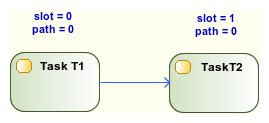
\includegraphics[width=\textwidth]{imgs/UML_SEQ_TSKS.png}
				\caption{Sequential tasks T1 and T2 are in different time slots.}
				\label{fig:UML_SEQ_TSKS}
        \end{subfigure}        
        \quad %\quad, \qquad, \hfill
        \begin{subfigure}[b]{0.4\textwidth}                
                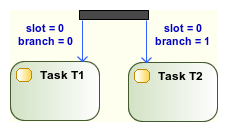
\includegraphics[width=0.8\textwidth]{imgs/UML_PAR_TSKS.png}
				\caption{Interleaved tasks T1 and T2 are in different time paths.}
				\label{fig:UML_PAR_TSKS}
        \end{subfigure}%
          
\end{figure}

Other supported behaviours are: alternative execution (E1|E2), optional execution (opt(E1)) and conditional execution (try(E)?E1:E2). For alternative execution, or XOR, a parameter in the model defines which alternative from a set of two or more is selected for analysis. Figures~\ref{fig:UML_ALT_TSKS} and~\ref{fig:PRISM_ALT_TSKS} illustrate the PRISM model and corresponding UML activities for alternative tasks T1 and T2.

\begin{figure*}[ht]
\centering
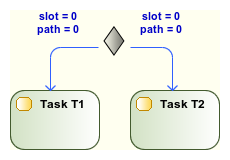
\includegraphics[width=0.4\textwidth]{imgs/UML_ALT_TSKS.png}
\caption{\detokenize{Alternative tasks T1 and T2 can be selected for analysis.}}
\label{fig:UML_ALT_TSKS}
\end{figure*}

\begin{figure*}[ht]
\centering
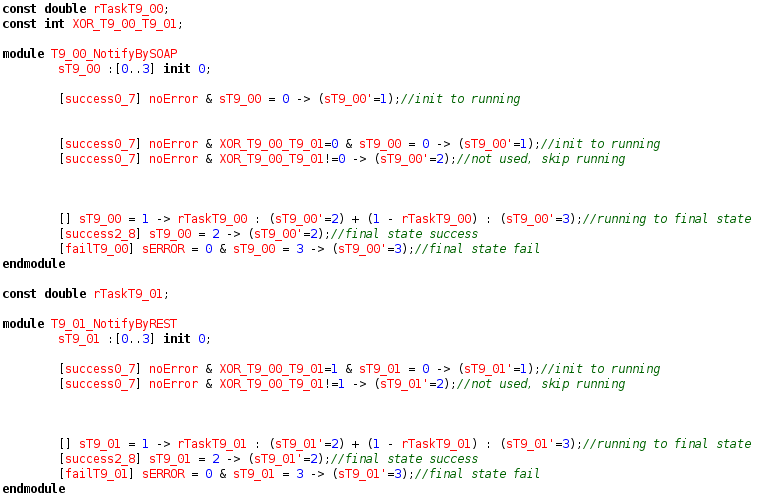
\includegraphics[width=1\textwidth]{imgs/PRISM_ALT_TSKS.png}
\caption{Alternative tasks T9.1 and T9.2 as DTMC modules with additional integer parameter used for selection.}
\label{fig:PRISM_ALT_TSKS}
\end{figure*}

Similarly to alternative execution, optional tasks are enabled by an additional parameter in the model. Figures~\ref{UML_OPT_TSK} and~\ref{fig:PRISM_OPT_TSK} illustrate the PRISM model and corresponding UML activity for optional task T17.2.

\begin{figure*}[ht]
\centering
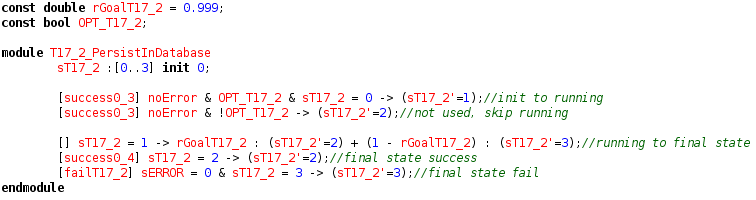
\includegraphics[width=1\textwidth]{imgs/PRISM_OPT_TSK.png}
\caption{An optional task T17.2 as a DTMC module with additional boolean parameter.}
\label{fig:PRISM_OPT_TSK}
\end{figure*}

Finally, labels are used to condition the execution of tasks to the success and failure of a third task. Figures~\ref{UML_TRY_TSKS} and~\ref{fig:PRISM_ALT_TSKS} illustrate the PRISM model and corresponding UML activities for conditional tasks T9.00 and T9.01.

\begin{figure*}[h!]
\centering
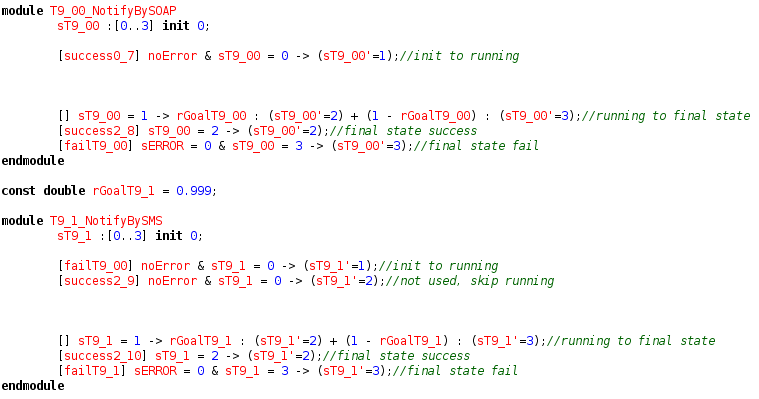
\includegraphics[width=1\textwidth]{imgs/PRISM_TRY_TSKS.png}
\caption{Conditional tasks T9.00 and T9.1 as DTMC modules.}
\label{fig:PRISM_TRY_TSKS}
\end{figure*}

Cardinality is also supported by the runtime regex specification. In our proposal, execution cardinality is simply represented by n modules with subsequent time slots (E+n) or by modules with synchronized initial transitions and followed by interleaved transitions (E\#n). Figures~\ref{fig:CRGM_TO_DTMC} and \ref{fig:PRISM_TRY_TSKS} illustrate different tasks behaviours.

%Listing~\ref{ls:MPERS_DTMC} presents the DTMC model for the MPERS.

%To illustrate our proposal for NFR verification of a single alternative, we selected the local goal G5 that defines the state where emergency rules are updated without major system interruption. Table~\ref{tab:MPERS_NFR} has a non-functional constraint for this goal that specifies the minimum

%Table~\ref{tab:MPERS_DTMC_SLOTS} presents the time slots, paths and other dynamic aspects of MPERS leaf-tasks.

% Please add the following required packages to your document preamble:
% \usepackage{booktabs}
\begin{table}[h]\label{tab:MPERS_DTMC_SLOTS}
{\renewcommand{\arraystretch}{1.5}
\begin{tabularx}{\textwidth}{@{}lllllll@{}}
\toprule
\textbf{Task}  & \textbf{Time path} & \textbf{Time slot} & \textbf{Optional} & \textbf{Conditional} & \textbf{Alternative} & Cardinality \\ \midrule
\textbf{T15}   & 0                  & 0                  & false             & false                & false                & 1           \\
\textbf{T16}   & 0                  & 1                  & false             & false                & false                & 1           \\
\textbf{T17.1} & 0                  & 2                  & false             & false                & false                & 1           \\
\textbf{T17.2} & 0                  & 3                  & true              & false                & false                & 1           \\
\textbf{T18}   & 0                  & 4                  & false             & false                & false                & 1           \\
\textbf{T19.1} & 0                  & 5                  & false             & false                & false                & 1           \\
\textbf{T19.2} & 0                  & 6                  & false             & false                & false                & 1           \\
\textbf{T20}   & 0                  & 7                  & false             & false                & false                & 1           \\
\textbf{T21}   & 1                  & 7                  & false             & false                & false                & 1           \\
\textbf{T9.1}  & 2                  & 7                  & false             & false                & T9.2                 & 1           \\
\textbf{T9.2}  & 2                  & 7                  & false             & false                & T9.1                 & 1           \\
\textbf{T22}   & 0                  & 8                  & false             & false                & T24                  & 2           \\
\textbf{T23}   & 0                  & 9                  & false             & false                & T24                  & 1           \\
\textbf{T24}   & 3                  & 8                  & false             & false                & T22                  & 1           \\
\textbf{T25}   & 3                  & 9                  & false             & false                & T22                  & 1           \\
\textbf{T13.1} & 4                  & 0                  & false             & false                & false                & 1           \\
\textbf{T13.2} & 4                  & 0                  & false             & false                & false                & 1           \\
\textbf{T13.3} & 4                  & 0                  & false             & false                & false                & 1           \\ \bottomrule
\end{tabularx}
\caption{Dynamic aspects of the MPERS leaf-tasks in the DTMC model.}
}
\end{table}


\subsubsection{Gathering individual task metrics}

Leaf-tasks are not necessarily atomic system operations and are generally described with a high abstraction level. For instance, the MPERS task `Find active sensors' could be further decomposed in more granular tasks. As it is, MPERS leaf-tasks are not coupled to any platform, architecture and language used for implementation.

%The idea is to leave to analysts the decision concerning the granularity and abstraction level represented by the tasks that will be verified. For instance, the abstract task `find active sensors' could be decomposed in more granular and concrete tasks related to the platform, architecture and language used for implementation. 

The more abstract a task is, the more difficult is to obtain their individual metrics, as the trace between an abstract and the concrete system operation becomes less evident. Any NFR verification by the PMC technique requires further information about individual parts involved in the overall activity, e.g., the reliability, performance, power consumption, cost and other attributes for tasks in a workflow (high-level DTMC).

This is a key point in this approach, as it may seen too loose to couple a probabilistic verification to a goal model with a high-level operational representation of a system. But its feasibility becomes more clear if the metrics being verified are compatible with the abstraction level of the leaf-tasks in the goal model and individual task metrics are available or can be collected. 

Depending on the purpose of the goal modelling - from early requirements elicitation to detailed design in TROPOS, more granular specification of tasks behaviour can be provided by decomposition and auxiliary UML diagrams. This internal task behaviour specification can be used for individual task analysis of metrics such as reliability and power consumption. In contrast, tasks execution instances could be monitored using the original RMG conformance algorithms. This hybrid verification requires a concrete system implementation besides the RGM system model. 



%In Section~\ref{ssec:RGM-UML} we argued that the RGM could replace a corresponding high-level UML activity diagram for PMC verification. However, if internal task behaviour is to be evaluated for a given metric, a both activity and sequence diagrams could serve as input for the evaluation of individual task metrics using a similar PMC technique.



\subsection{Reasoning with Ex-Tropos}

The probabilistic verification of NFR, performed as part of the Validation \& Verification (VV) phase in RE, should anticipate (contextual) violations of non-functional requirements. Treating a detected violation at design time may correspond to actions such as making a different choice for underlying components used by this alternative's tasks, optimizing its behaviour specification or even the disposal of this alternative as a means to satisfy its goal if there is at least one other valid alternative. 

PMC technique also allows the identification of system alternatives with more influence on each metric through sensitive analysis.

\subsubsection{Variability in GORE}

The variability in goal models leads to more than one minimum set of tasks capable of fulfilling local or root goals. In OR-decompositions, at least one alternative is required and the maximum number of combinations is defined by $1 + 2^{(n-1)}$, with n the number of OR-decomposed goals/tasks. Therefore, the verification of all alternatives in a goal model with individual models may prove to be inefficient or infeasible if too many variation points exist in the model.

The PMC approach has already been explored for the verification of models with variability. Rodrigues et al. proposed a family-based verification of software product lines (SPL)~[RODRIGUES]. The main idea is to reduce the analysis effort and boost the feasibility of the SPL verification. In the proposed family-based verification, parameters in a PRISM probabilistic model generates a parametric formula for all products in the SPL for a given PCTL property. 

In our proposal, PCM verification follows the same principle of the SPL family-based verification. A parametric DTMC model should be generated from the RGM. Alternatives are selected by passing values to parameters. For instance, if both GPS and triangulation are available means for identifying the patient location, a parameter with values 0 or 1 will indicate which alternative is enabled for verification. 

%Eq.~\ref{eq:MPERS_RELIABILITY_FORM} defines the reliability formula for the root goal G1.

%\begin{equation}
%G1r=c^2\label{eq:MPERS_RELIABILITY_FORM}
%\end{equation}

A family-based PMC is useful for comparing each alternative with non-functional metrics as criteria to decide which one should be used by the system-to-be at design time or by the real system at runtime. At design time, this approach is analogue to the TROPOS contribution analysis. In both cases, a unique parametric formula evaluates a PCTL property corresponding to a non-functional metric.  %improve the example!


% or the verification tool should decide based on some probabilistic distribution setted by the analysts (probabilistic alternative selection, or PAS).

%In contrast, PAS provides verification for systems that include variability in its design. The verification of NFR metrics for these systems depend on how each alternative is selected during system operation.

\subsubsection{Context selection}

As in the contextual goal model, contexts may limit which alternatives are adoptable. This effect must be considered in a realistic verification. As a novelty, our approach for the verification of non-functional metrics through PMC will also include variable contexts of operation and their effects in the verification model. Two different approaches for context selection may be employed: 

\begin{itemize}

\item \textit{Deterministic context selection, or DCS}: one context is selected by the analyst before the verification. Context effects in the verification model should be activated and cause the evaluation result to correspond to the selected context.
\medskip

\item \textit{Probabilistic context selection, or PCS}: a probability distribution will define the likelihood of a context to be selected and the corresponding context implications in the verification model to be activated.  

\end{itemize}

Both approaches are complementary as the first verifies the selected alternative for one context at a time and the last verifies a realistic scenario with multiple possible contexts. 

\subsubsection{Context-alternative selection}

Table~\ref{tab:DAS_PAS_DCS_PCS} summarizes each verification approach and possible combinations.

% Please add the following required packages to your document preamble:
% \usepackage{booktabs}
\begin{table}[h]\label{tab:DAS_PAS_DCS_PCS}
{\renewcommand{\arraystretch}{1.5}
\begin{tabularx}{\textwidth}{@{}l|XXX@{}}
\toprule
             &                                                         & \textbf{DAS}                                                                                                      & \textbf{PAS}                                                                                                     \\ \midrule
             &                                                         & A single alternative is selected by the analyst.                                                                  & Alternative selection follows a probabilistic distribution.                                                      \\
\textbf{DCS} & An unique context is selected by the analyst.           & Alternative selection by the analyst is limited by the selected context.                                          & Probabilistic alternative selection is limited by the selected context.                                          \\
\textbf{PCS} & Context selection follows a probabilistic distribution. & Alternative selection by the analyst may fail according to the probability of selecting an incomplatible context. & Probabilistic alternative selection may fail according to the probability of selecting an incomplatible context. \\ \bottomrule
\end{tabularx}
}
\caption{Description of the different approaches for verifying a system with variable alternatives and variable contexts.}
\end{table}

If the context selection is deterministic (DCS), there is no reason for verifying an alternative that is known to be incompatible with the selected context. Therefore, only adoptable alternatives must be verified. In opposition, if context selection is probabilistic, that alternative may still be valid in other contexts, hence it must be included in the multi-context evaluation. For instance, the patient location identification through GPS (alternative) will certainly fail if the GPS signal is not available (context). Thus, the DAS-DCS combination checks one compatible context-alternative pair at a time, while DAS-PCS combination leads to the verification of multiple context-alternative pairs at the same time.

The idea behind a probabilistic context selection is to emulate a realistic scenario in which the context of operation varies and the system must avoid requirements violations by  having an adoptable alternative for each context. This holistic evaluation provides measures weighted by the probabilistic context distribution. For instance, if GPS signal is available 70\% of the time and triangulation is available 90\% of the time and if each method has its own reliability, namely rGPS and rTRI, the reliability of high-level task `identify patient location' is defined by the expression 0.9*rGPS + 0.1*0.7*rTRI, considering that GPS has priority over triangulation. 


\subsubsection{Discrete-time Markov chain model}



\subsubsection{Reliability verification}

Transition probability between running to final success state is described by the individual reliability of the corresponding task, namely rTask. 

\subsubsection{Power consumption verification}

%The same principle is applied to the PAS combinations. Incompatible alternatives are removed from the selection list if the context for which they are incompatible is fixed. Or, if context selection is probabilistic, for each context the verification model should be able to avoid the probabilistic selection of incompatible alternatives. This simulates the self-adaptive capability of systems that are designed to tolerate context changes.

%This section is divided in preliminary conceptual explanation about the

\subsection{From NFR to PCTL properties}

The estimation of attributes through PMC technique is limited to those that a probabilistic model may evaluate. Dependability attributes have an abstract definition that must be associated to a concrete and verifiable PCTL property. To demonstrate our approach, we verify the MPERS model for the following attributes:

\begin{itemize}

\item \textbf{Reliability}, represented by the probability of a successful execution of all the activities involved in fulfilling leaf-goals of a certain system alternative. It is also know as the \textit{reachability} as the describes the probability of reaching a final and successful system state. 
\bigskip

\item \textbf{Availability}, represented by the power consumption estimation to maximize the time that the system will remain operational depending only on its battery. This attribute is well related to mobile computing. 
\medskip

\end{itemize}


each task has its own states, including the failure and the success states. Many factors may contribute to the correctness or the failure of system tasks, including internal and external events. The probability of a successful task execution defines its reliability. 

In a complex workflow of tasks with different rel 

In order to be successful, tasks depend on the proper interaction among the components 

seen as an activity diagram and be used to generate a probabilistic model in PRISM language. This allows the model checking of the corresponding goal model as a set of activities for which temporal and other behaviour aspects are specified by the runtime regex of the RGM.

\section{Treating NFR Violations}

\begin{itemize}

\item Making a different choice for underlying components: In some cases the replacement of a technical component for another of the same class can improve the quality of how they achieve their goal. For instance,
\medskip

\item Behaviour optimization: The quality may also depend on the pattern used for the activities execution. The specification of a different pattern may eliminate the non-functional violation. 
\medskip

\item Contextualizing the alternative: An alternative may only violate a NFR in specific contexts. In this case, different valid alternatives may be used according to the context of operation.
\medskip

\item Alternative disposal: If the alternative is in absolute violation or if its validity is restricted to contexts that have at least one other valid alternative, this branch can be eliminated from the model.

\end{itemize}

Dependability analysis is used to provide information about different dependability attributes related to system failures. These metrics may be specified as non-functional requirements for isolated system functionalities or for the whole system. Instead of softgoals, we use meta-requirements over functional goals with clear-cut quantitative criteria such as `99.999\%' reliable - a probabilistic value to make it compatible with the PMC estimation results.

To perform the , we focus on dependability related metrics that should be estimated and compared to their required constraint values through quantitative analysis. Sensitive analysis to reveal how different system parts contribute to the overall value of those attributes. Sensitive analysis may be considered analogous to the original GORE contribution analysis.
